\section{Result}
\label{result}

To compare the results shown in the article \cite{liu2010}, we test our implementation for all the cases reported in that article. All the tests reported below are executed on Pianosa\footnote{Pianosa web site: \url{http://pianosa.di.unipi.it/Home_pianosa/html/info.html}}, the Computer Science Department's Cluster in Pisa. The cluster is composed by 24 homogeneous nodes. The nodes are 800 Mz Pentium III with 1GB of main memory and they are connected together through a Fast Ethernet interconnection network. On that cluster, we installed an Hadoop 0.20.2 framework. The configuration parameters are set to default, so, the maximum number of task per node is set to 2 and the number of replication is set to 3. In our configuration, we decide to place the secondary node and the job traker in cluster interface node that is not used also as task tracker. Only other 21 nodes are available as slave, cause to momentarily unavailability of the other nodes.

The data used in the test are generated by two generators written in Matlab: one for the matrix A and other one for the matrices W and H. Both generators produce positive elements Gaussian distributed. The first one is a sparse matrix generator and its sparsity factor can be tuned through an input parameter. The second one, instead, is a complete matrix generator. For our tests, we fix the $m$ and $n$ parameters respectively to $105000$ and $20000$.

For all the test we did, the reduce task number is set to $ 1,8 * number\_of\_worker$, where is possible\footnote{Note: the phase 3 and 4 have a fixed number of reduce task}. This choice has been driven by the Hadoop User Guide that suggest to set the reduce task number to $$ mapred.map\_reduceMaximumTask * number\_of\_worker * C $$ where C is a constant choose in the range $[ 0.9, 1.8]$. For a value chosen in that range, it claim that the number of reduce tasks is optimal. In our experiments, we set that constant C to 0.9. Also for the first  W/H update, the input number can be set in the proper way. In fact, the External Phase classes (that convert the input data from text to sequence) allow to specify how many reducer tasks must be used. In that way, an equal number of file are produced.

The first test battery done tests how the computation scales in relation to the the size of the data submitted. So, we study how the performances change varying the sparsity factor of the A matrix and setting different k values. In the first test, the number of non-zero elements in the sparse matrix has been changed between $5000000$ and $80000000$ elements while the k parameter remain fixed to 10. In the second one, instead, the k value has been varied between 10 and 125 while the non zero element of the A matrix has been fixed to $16500000$.  Both tests have been executed with 16 slave nodes for three iterative updates. The iterative update mean values of W/H matrices is reported in the figure \ref{DeltaVar}  and \ref{kVar}. 


\begin{figure}[th]
	\centerline{
		\mbox{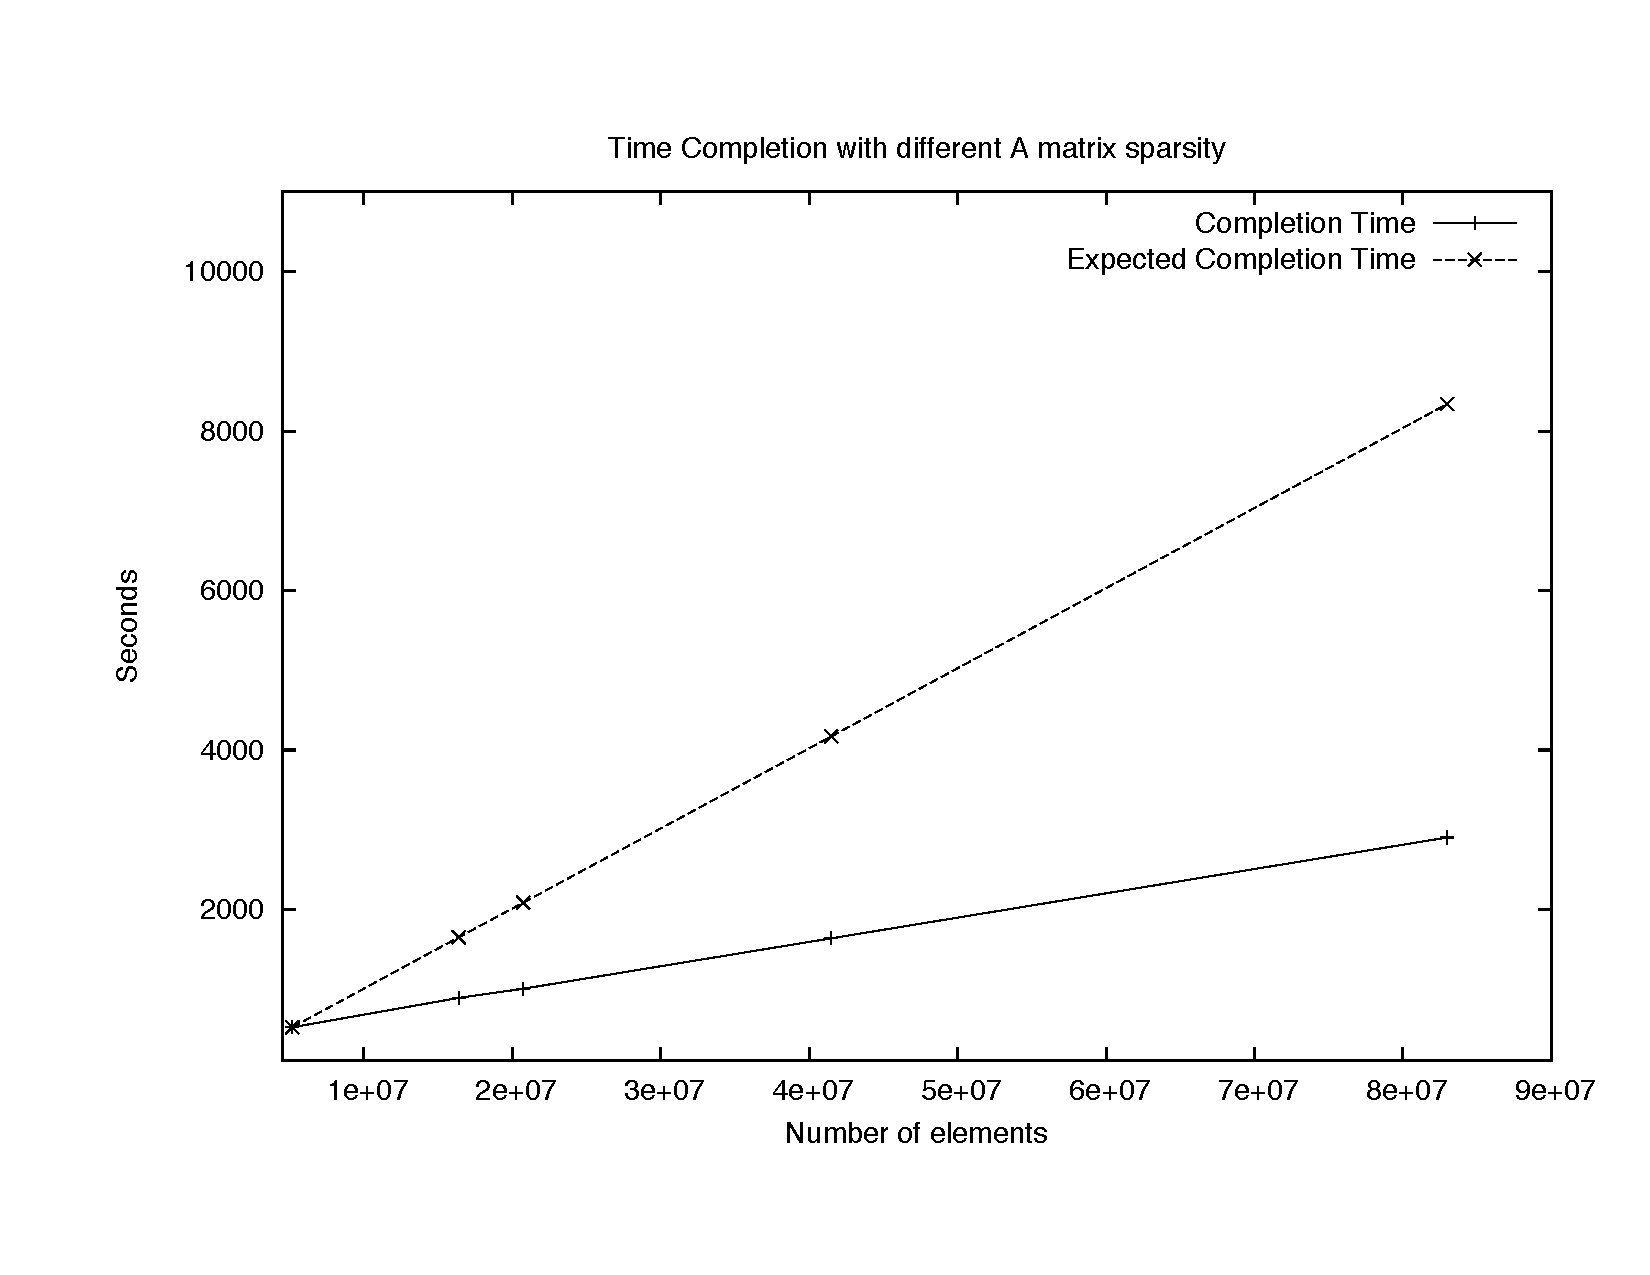
\includegraphics[scale=0.48]{HadoopTest/PsFiles/DeltaVar.pdf}}
	}
	\caption{Time Completion with different A matrix sparsity} 
        \label{DeltaVar}
\end{figure}

\begin{figure}[th]
	\centerline{
		\mbox{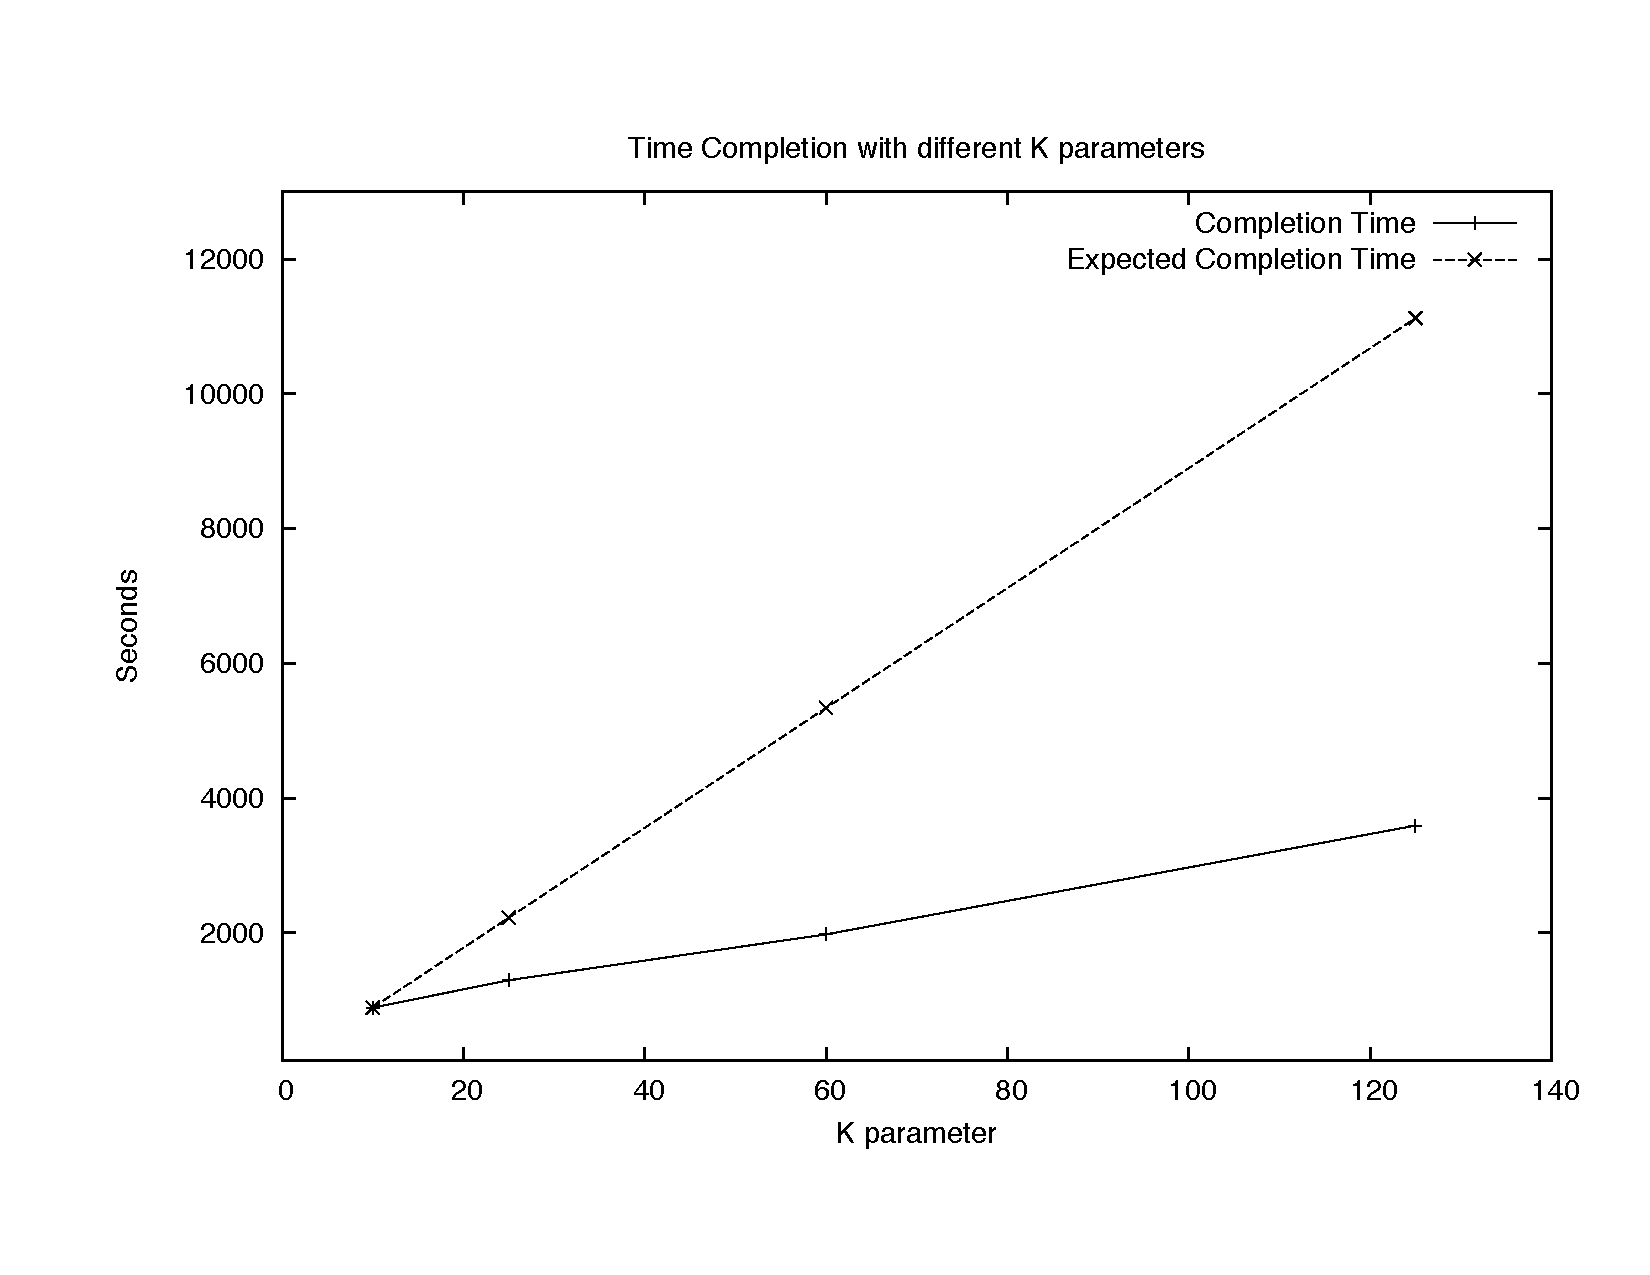
\includegraphics[scale=0.48]{HadoopTest/PsFiles/kVar.pdf}}
	}
	\caption{Time Completion with different K parameters} 
        \label{kVar}
\end{figure}


As we can see from both graphs, the behaviour of the test show a sub-linear dependencies from the size of the input data. \\

The second test battery points to examine the behaviour of the implementation when the parallel degree of the computation vary in the range $[1, 21]$. The results of the test are reported in the figure \ref{NTime}  and \ref{NScal}. The first graph focus the attention on the completion time while the second one on the scalability.


\begin{figure}[th]
	\centerline{
		\mbox{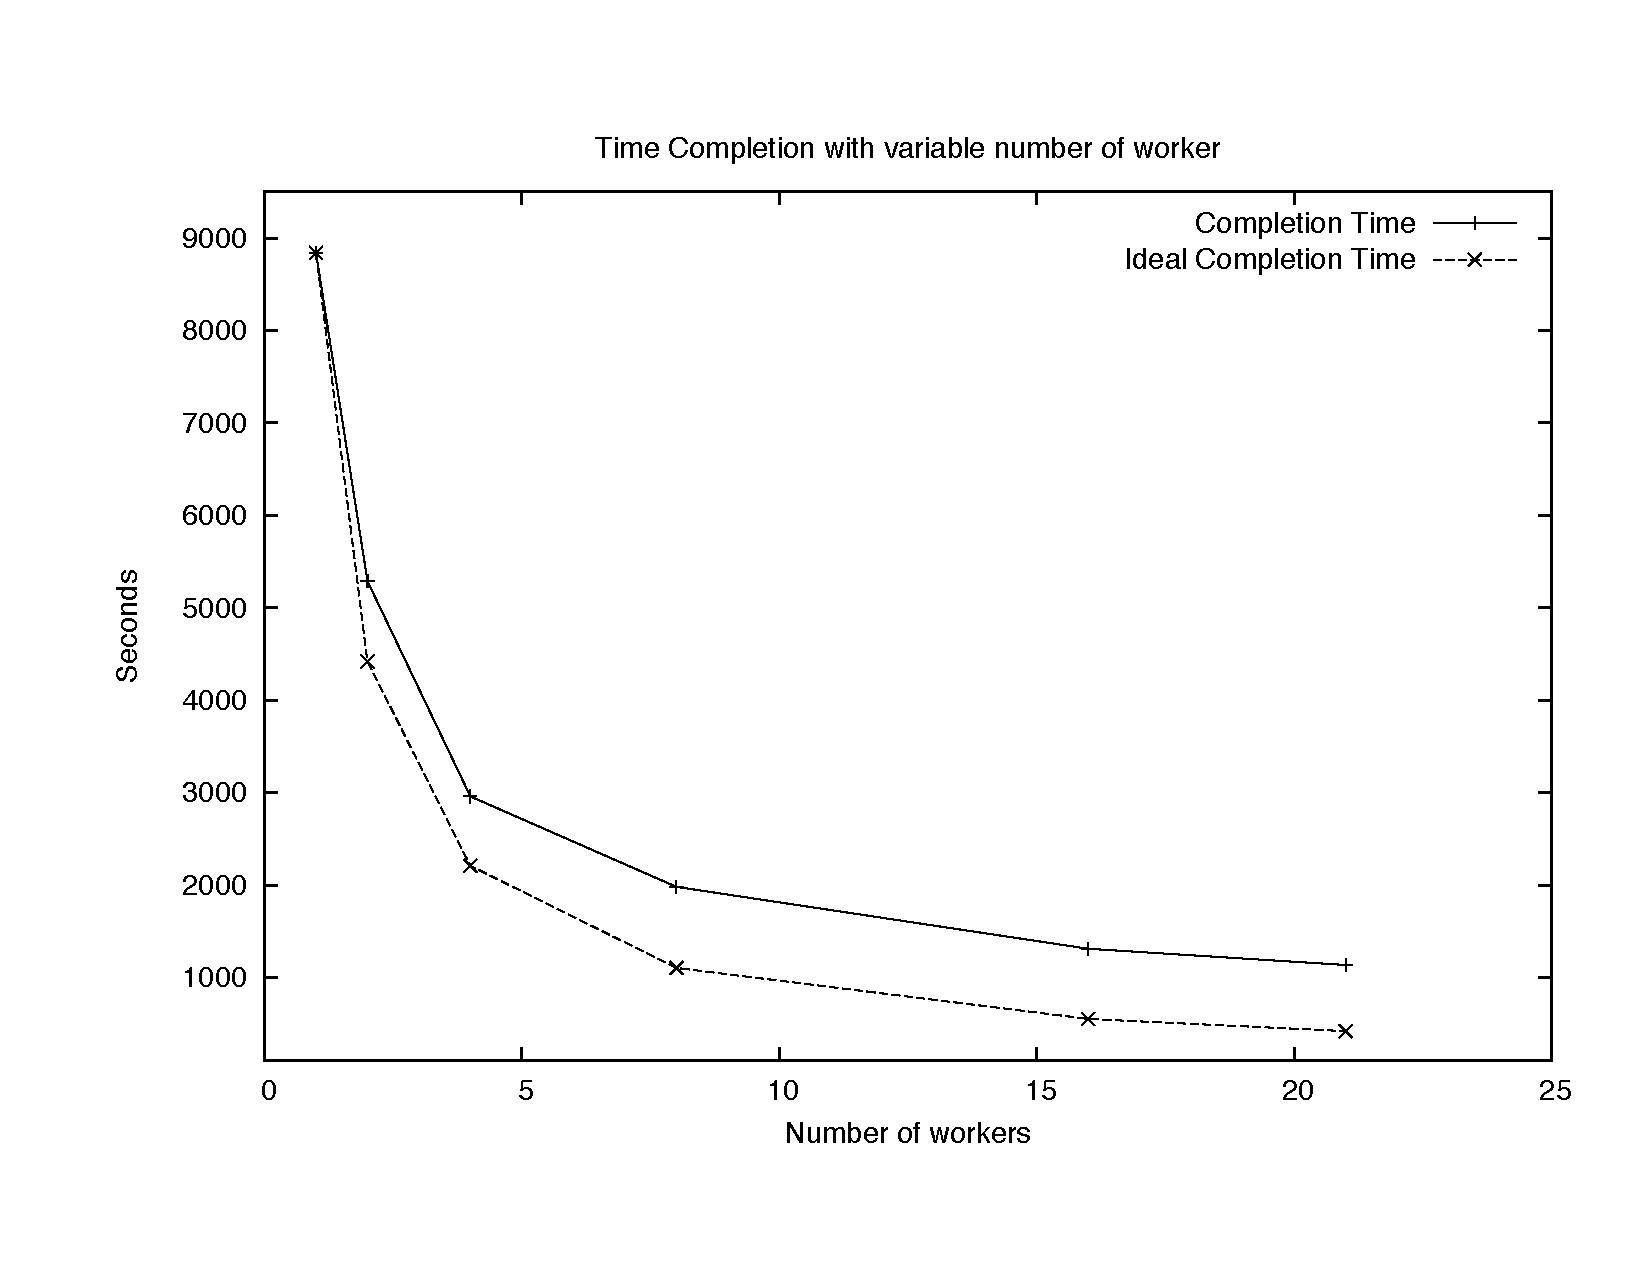
\includegraphics[scale=0.48]{HadoopTest/PsFiles/NTime.pdf}}
	}
	\caption{Time Completion with variable number of worker} 
        \label{NTime}
\end{figure}

\begin{figure}[th]
	\centerline{
		\mbox{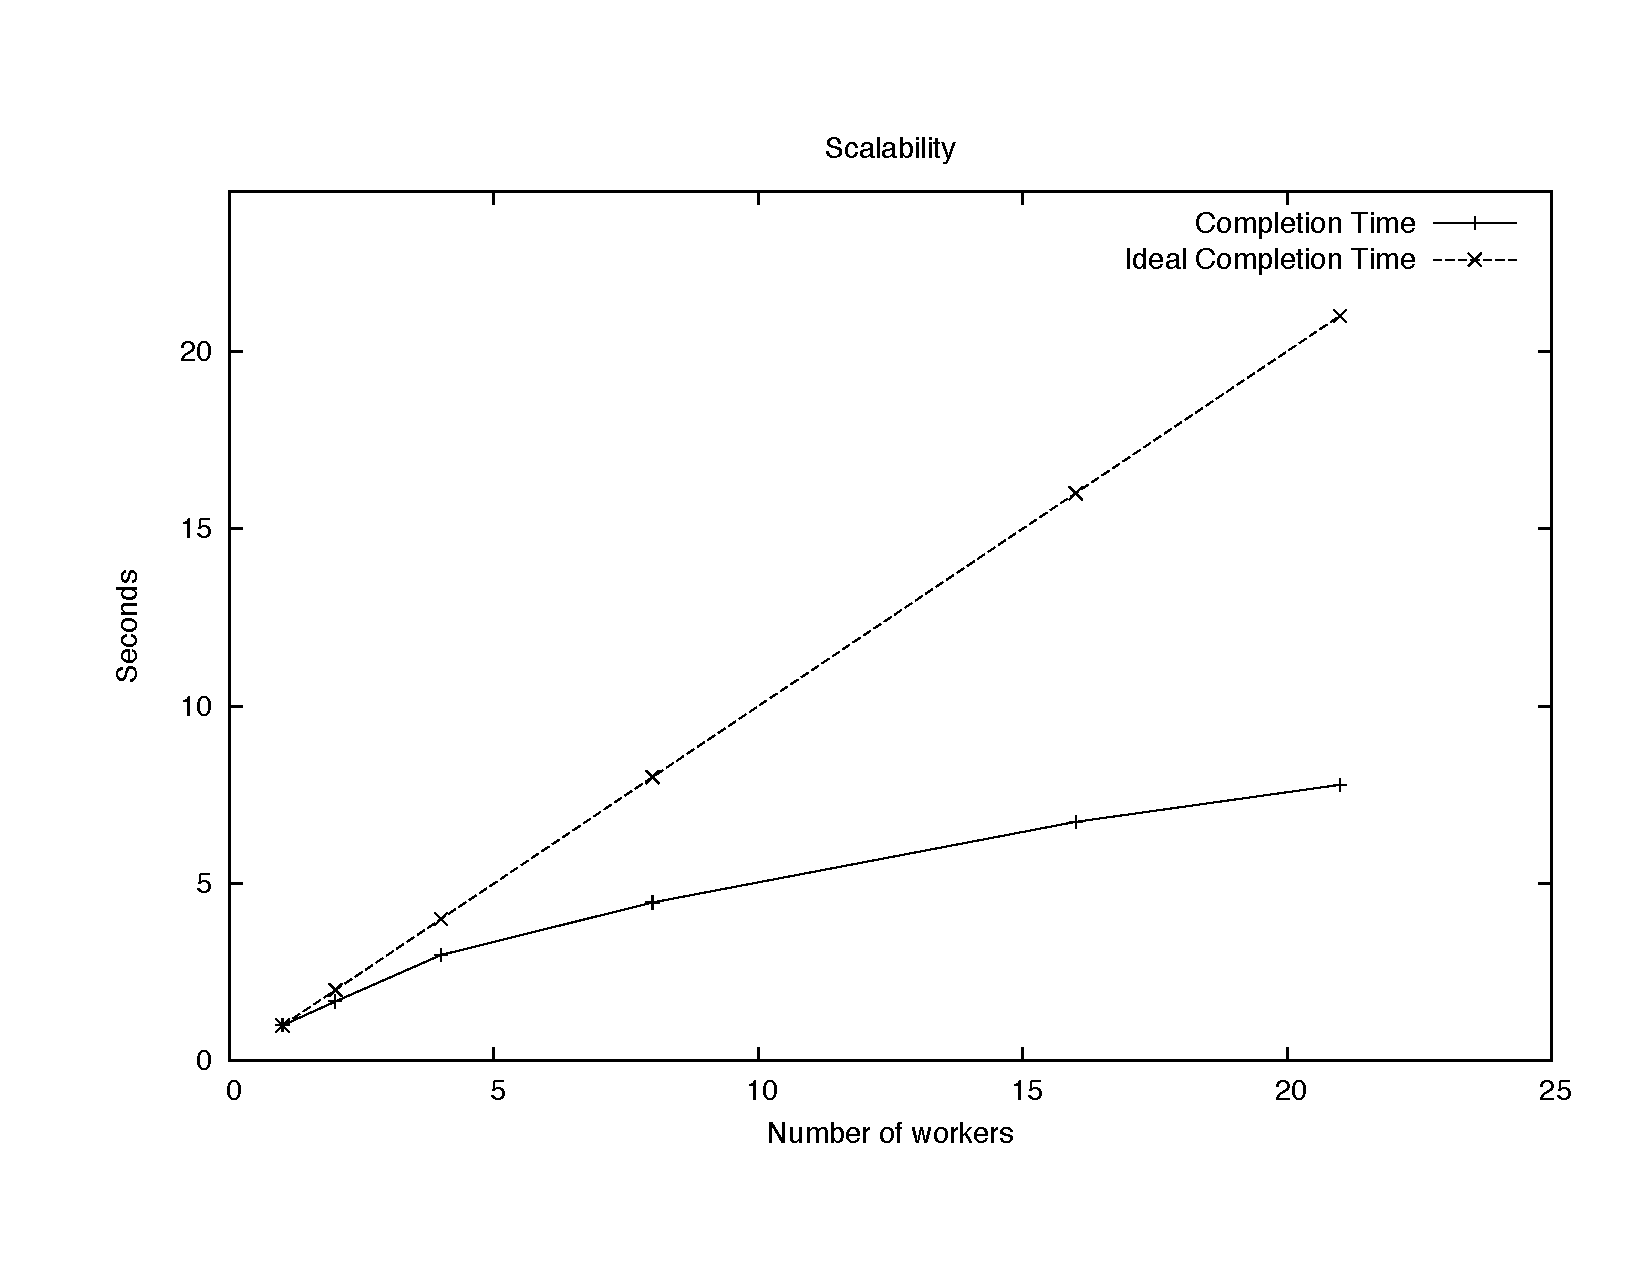
\includegraphics[scale=0.48]{HadoopTest/PsFiles/NScal.pdf}}
	}
	\caption{Scalability} 
        \label{NScal}
\end{figure}

As we can see.....